\setcounter{chapter}{3}
\setcounter{section}{0}
\setcounter{subsection}{0}
\chapter*{Results}
\section{Current Workflow}
The current workflow in MERIT.jl was designed to be simple and approachable without much background knowledge about how
Julia or the underlying library works. Shown below is the full workflow needed to generate a plot from the data:
\lstinputlisting[language=Julia]{../../src/GettingStarted.jl}
A user would first instantiate the BrestScan struct and assign the data types that would be used throughout the
processing pipeline. The first type sets the data type and thereby the precision of the points composing the imaging
domain, the antenna locations and the frequency divisions. This can be any datatype that is a subset of type Real. The
second type controls the data type of the signal matrix containing the data collected from each antenna. This can be any
type that is a subtype of Number allowing for time-domain (Real) signals or frequency-domain (Complex) signals. The
third type controls the data type of the channels, and it can be any type that is a subtype of Integer. The choice of
data type here has no accuracy impact on the final result and it is recommended to choose an Unsigned Integer data type
that is big enough to index all the antennas. The next step would be to generate the imaging domain, this is
accomplished using the \lstinline[language=Julia]{domain_hemisphere!} function. This accepts the resolution and the
assumed or calculated radius of the breast. The user would then have to make use of the
\lstinline[language=Julia]{load_XXX!} functions to load the data into the relevant fields of the struct. These functions
assume the data is contained in a CSV file and contain no headers. The user then populates the relevant fields with
their chosen beamformer and delay function. At this stage, the user can then pass the whole struct to the
\lstinline[language=Julia]{beamform} which will beamformer the provided signals into a set of data that can then be
visualized as demonstrated towards the end of the code block above. Overall the entire workflow can be seen in Figure
\ref{fig:MERITWorkflow}.

\begin{figure}[h!]
    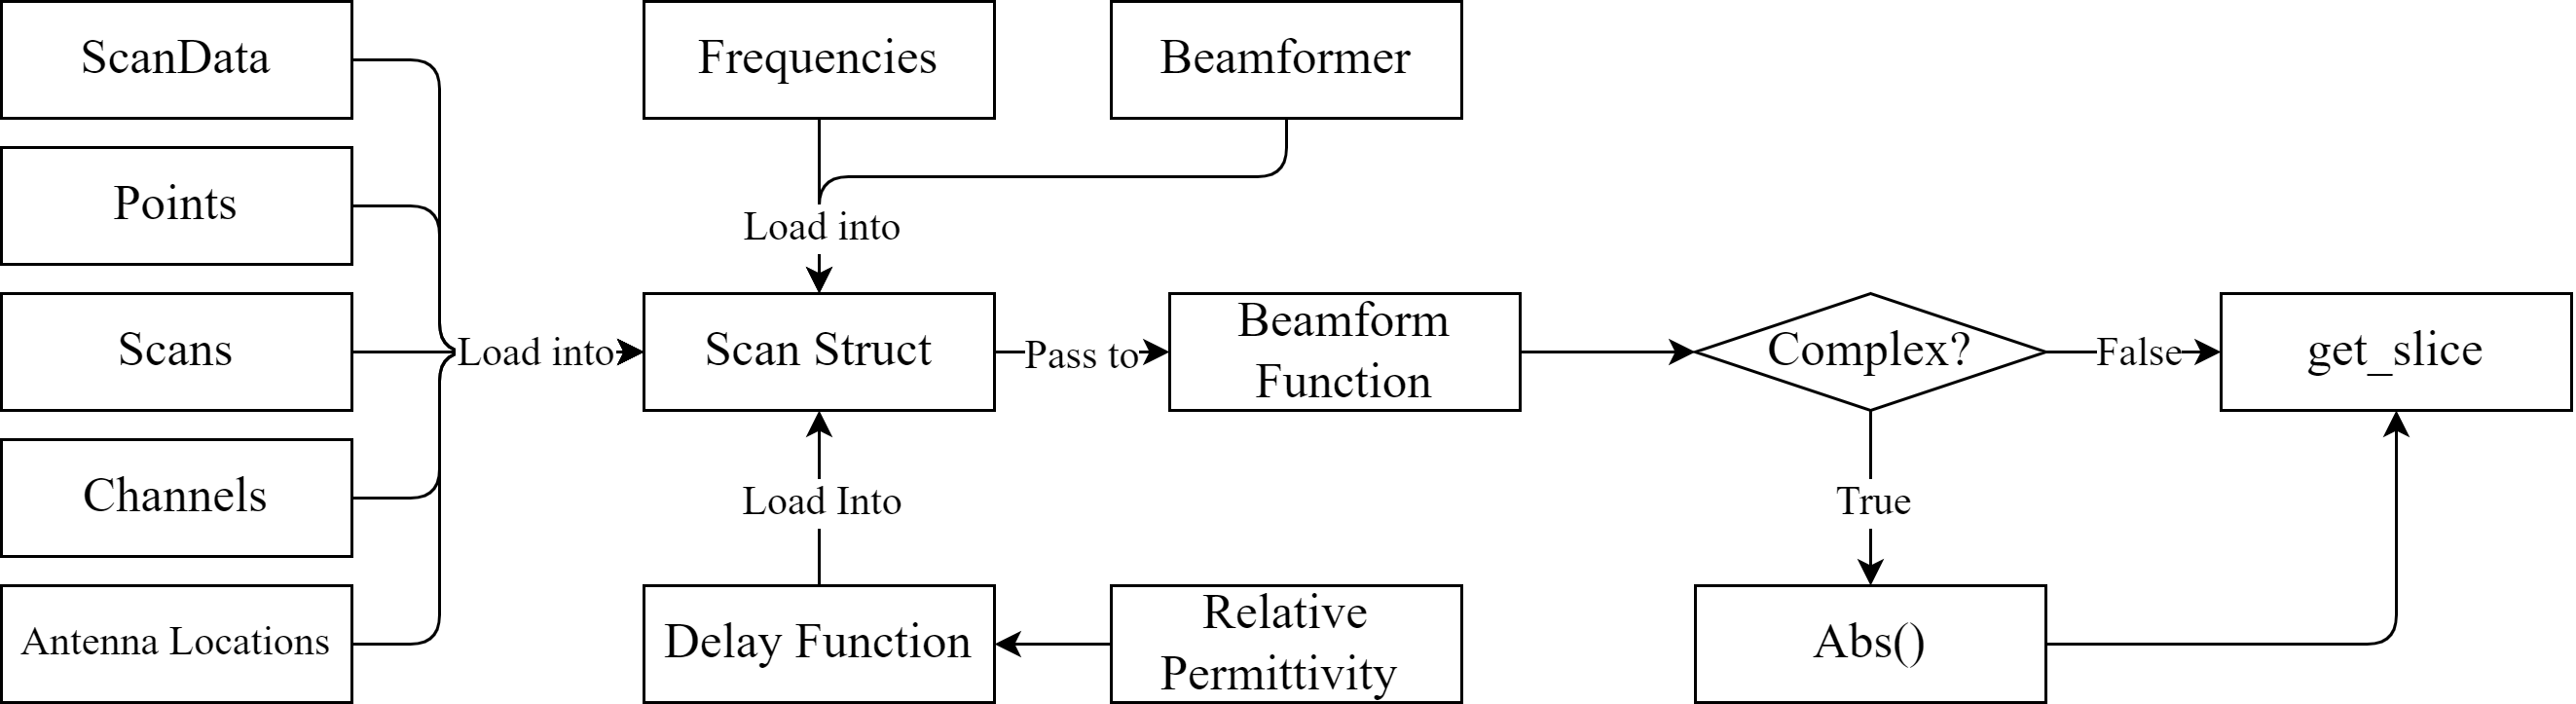
\includegraphics[width=1\textwidth]{MERITWorkflow.png}
    \centering
    \caption{The entire MERIT.jl Workflow} 
    \label{fig:MERITWorkflow}
\end{figure}

This workflow exemplifies how easy it is to use the MERIT.jl library. The function names were deliberately chosen to be
verbose and conform to established nomenclature in the field so that anyone who wants to use the library can understand
what each function does without having to delve into the source code. In this way, the MERIT.jl library is somewhat self
documenting. Additional information is provided above each function in the form of docstrings which can be used with the
help function built into the Julia REPL. This was done in a bid to lower the prerequisite knowledge needed to use the
library, thereby fulfilling one of the goals of MERIT.jl which was to create an open and acessible library. 

\subsection{MERIT.jl Results}
The library was benchmarked against the MATLAB implementation created by Prof O'Loughlin et al to ensure that the
results provided by MERIT.jl are provably correct. Both implementations were given the same data, B0\_P3\_p000.csv and
B0\_P3\_p036.csv. Rotational subtraction was performed on these in both libraries to reduce the presence of skin
reflections in the data as mentioned before. The data was then processed according to the processing pipeline
recommended by both libraries, the result of which can be seen below in Figure \ref{fig:MERITResults}. It should be noted that the \lstinline[language=Octave]{imshow} function was used in MATLAB to plot the image. This had
the effect of reflecting the image across the x-axis and also slightly stretching the image along the x-axis, however,
the matrix holding the image data still shares the same layout as the image matrix in Julia so a numerical
comparison between the two could be performed. The averaged MSE proved to be an excellent choice as a numerical
comparator, due to the squaring operations in the MSE formula any small differences would be greatly magnified in the
error. This is desirable when the goal is to see if MERIT.jl can provide output that is similar to its MATLAB
counterpart. Computing the averaged MSE between the two images yielded an error of $8.4417 \times 10^{-7}$ which is well
within the accuracy of a float, making it effectively identical to the images produced by MATLAB. This shows that the
Julia library in its current state provides a viable alternative to the MATLAB implementation for frequency domain
analysis.

\begin{figure}[t]
    \begin{tabular}{cc}
        \subfloat[MERIT.jl Output]{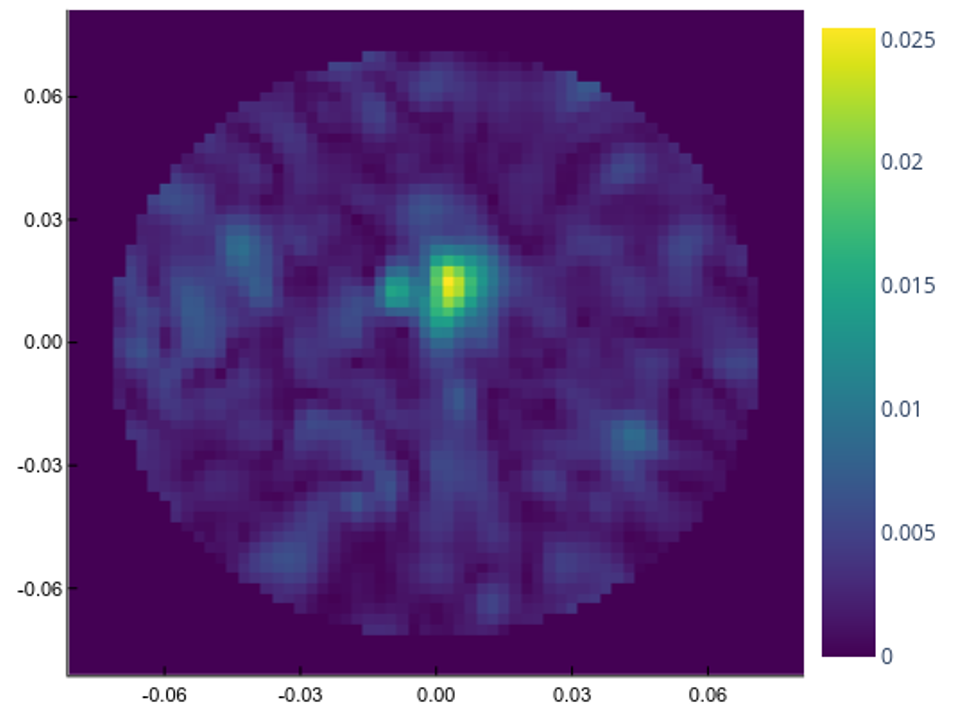
\includegraphics[width=0.45\linewidth]{JuliaOutput.png}}&
        \subfloat[MATLAB Output]{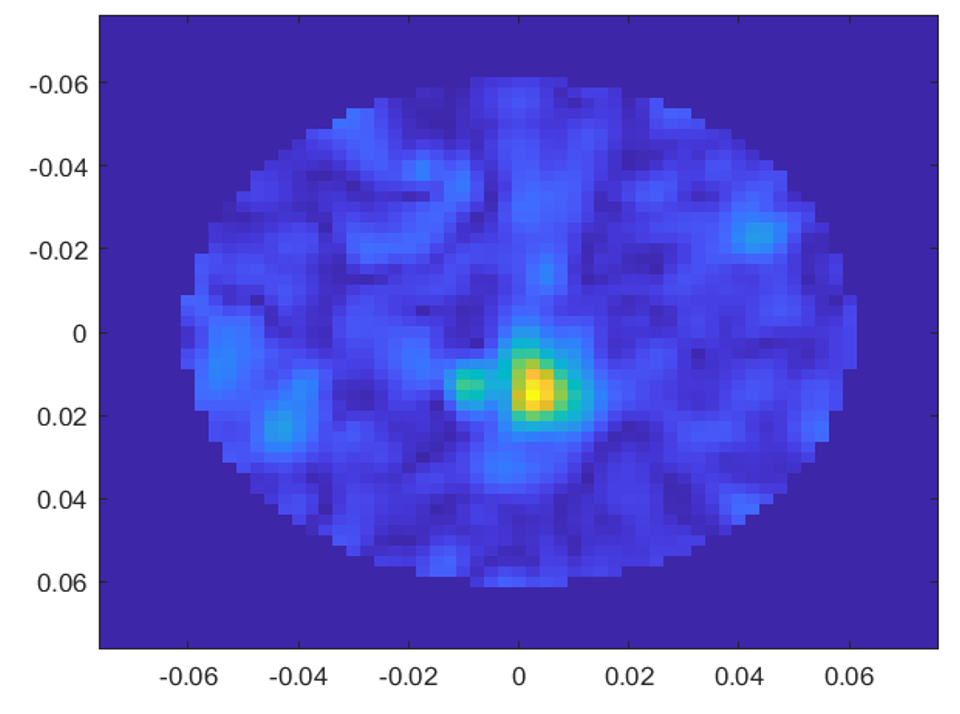
\includegraphics[width=0.45\linewidth]{MATLABOutput.png}}
    \end{tabular}
    \label{fig:MERITResults}
\end{figure}


\subsection{Performance of MERIT.jl}
One of the requirements for MERIT.jl was that it had to be performant. Through the use of type stability, SIMD optimized
for loops and the disabling of array bounds checking, the library could process the provided data in 8 seconds. However,
after the addition of the Points data type for type safety, the processing time climbed to 12 seconds. While the overall
runtime is still acceptable, an increase of 3 seconds is less than ideal. While no official analysis has been conducted
to narrow down the cause of the slowdowns, I suspect that perhaps it may be down to unoptimized implementations of the
basic operators such as addition and squaring in the Points.jl library. It should also be noted that when running the
library, my laptop constantly ran into memory limits and had to write some memory to a swap file on disk. I believe that
moving memory in and out of this file might also be partly responsible for the increased runtime, however, further
research is necessary to determine a definitive cause. To capture the full performance characteristics of the library, a
scalability test was performed, in which the number of points, channels and frequency divisions were progressively
increased. This was performed in an automated manner using the functions provided by BenchmarkTools.jl
\cite{BenchmarkToolsJl}. The results from the benchmark suites were then exported to CSV files and analyzed in Excel to
judge the "Big O" notation of MERIT.jl.

\begin{figure}[h!]
    \begin{tabular}{cc}
        \subfloat[Unedited Points]{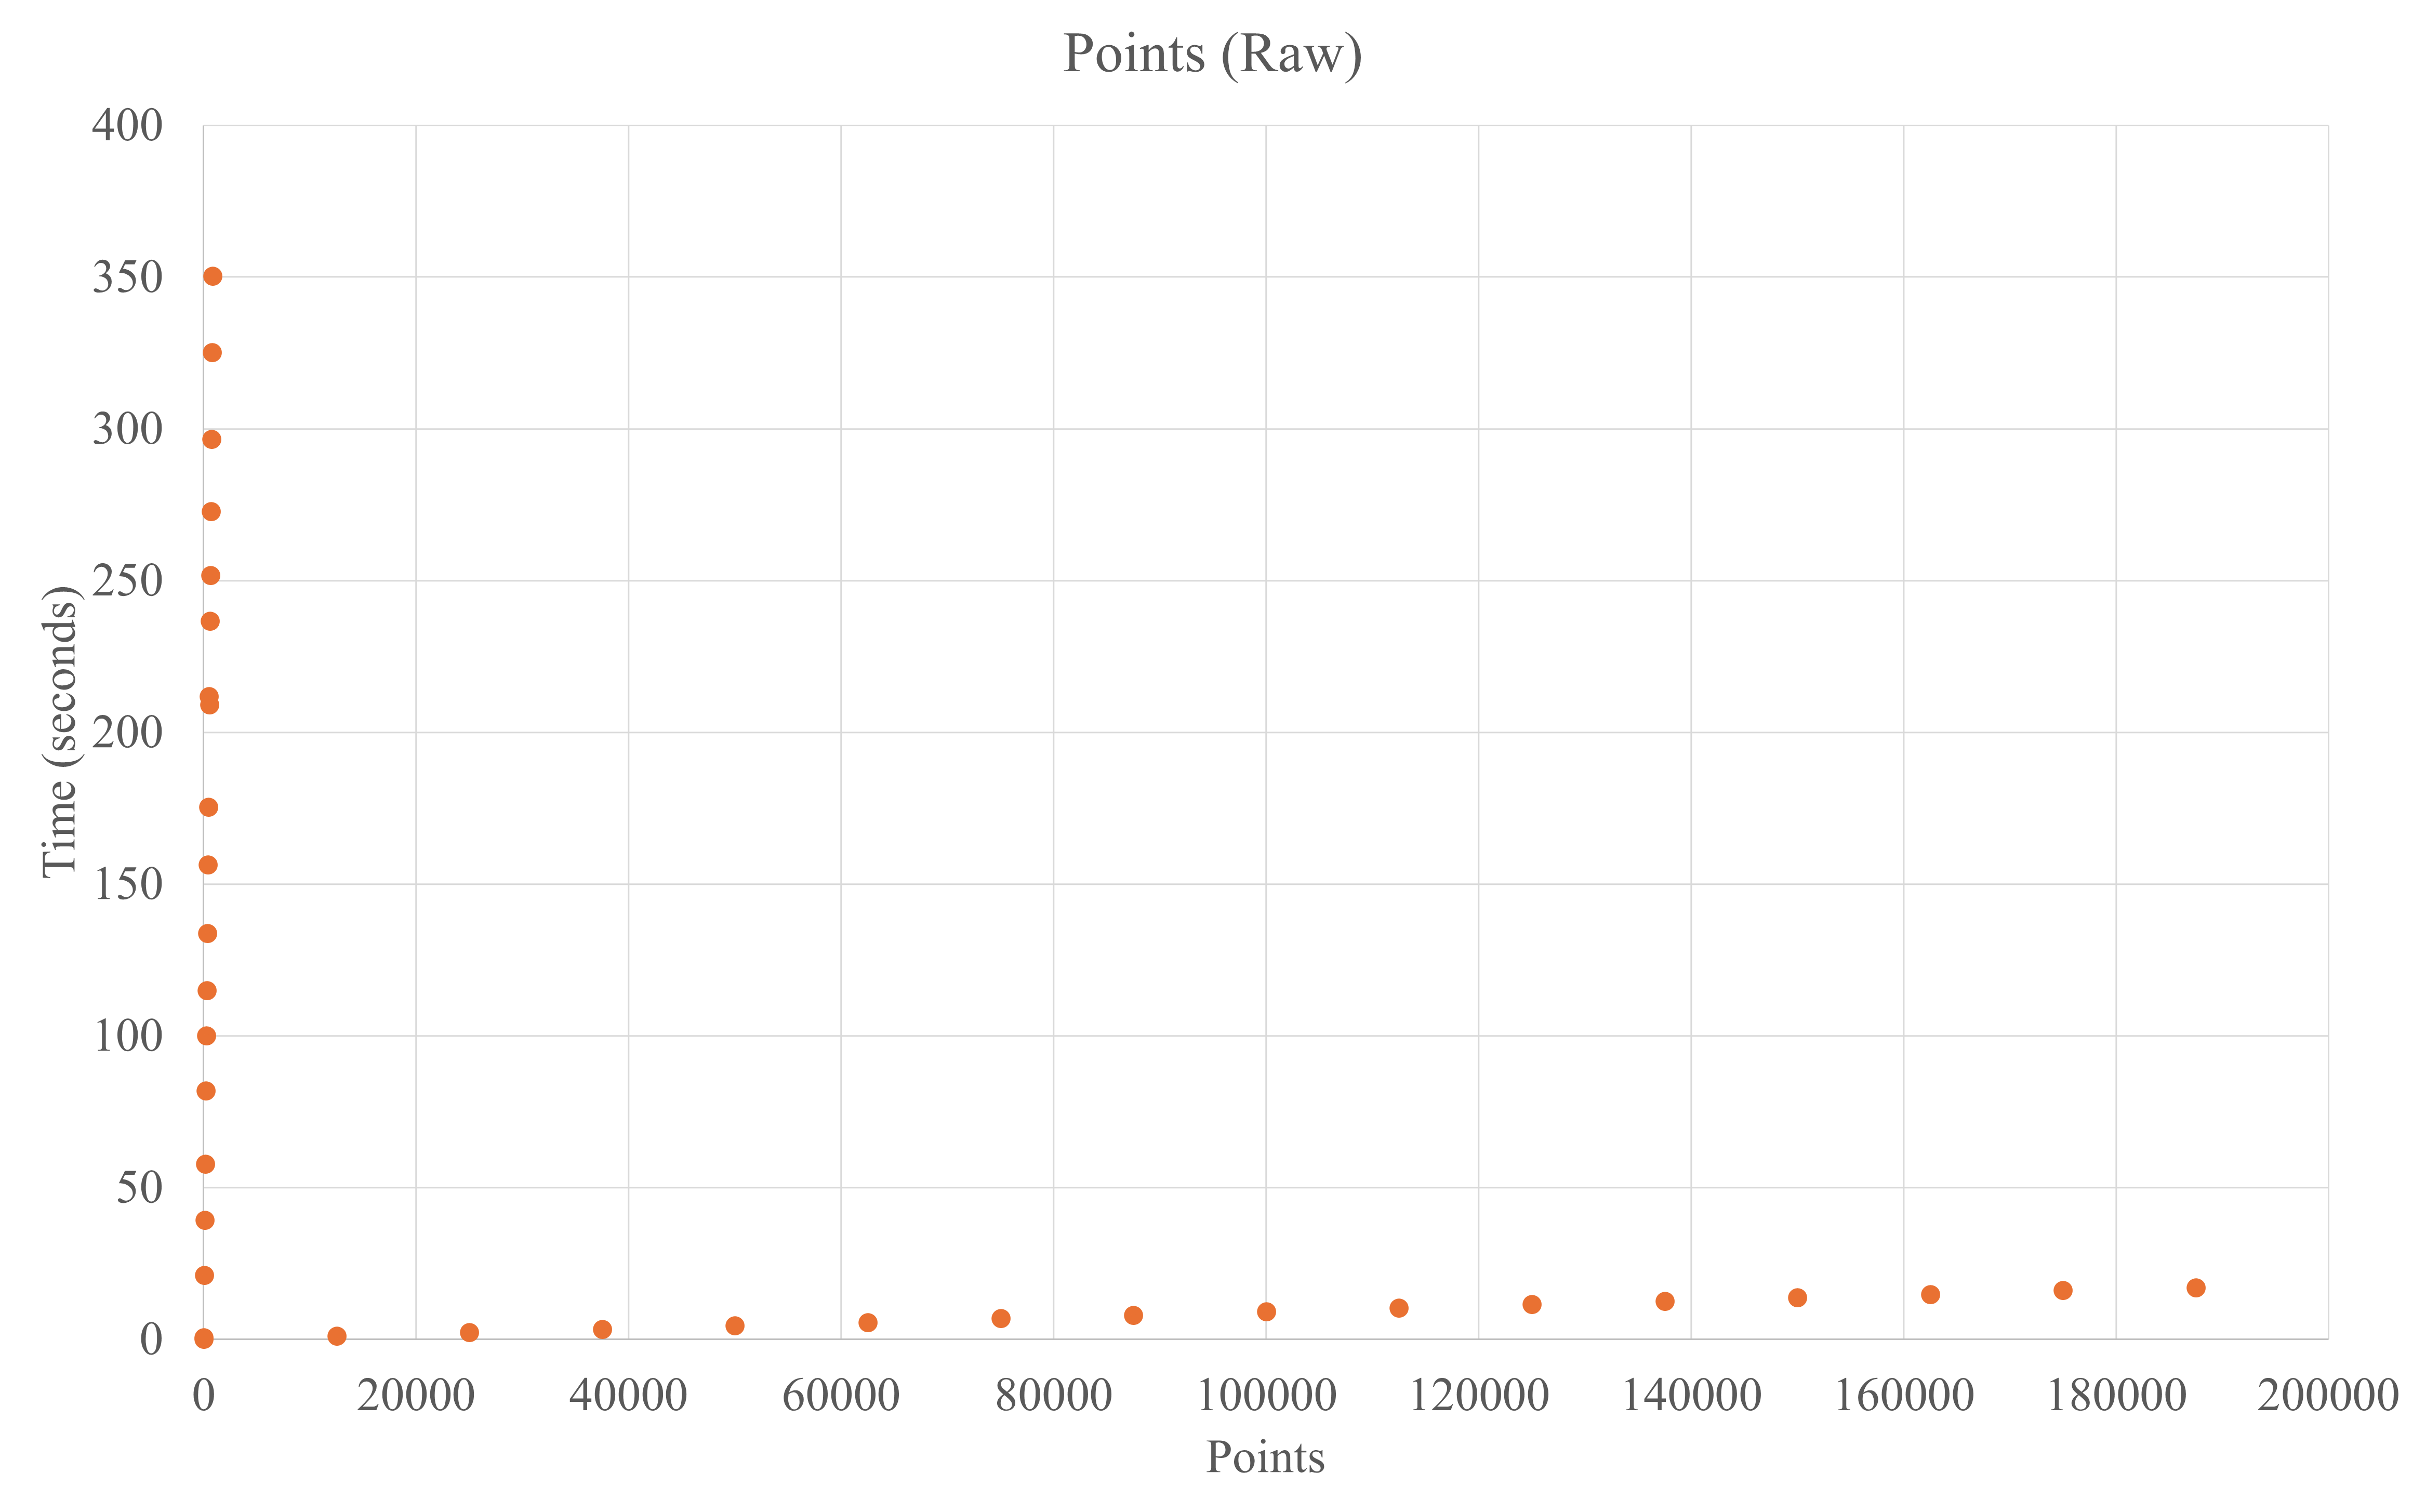
\includegraphics[width=0.45\linewidth]{PointsUnedited.png}}&
        \subfloat[Edited Points]{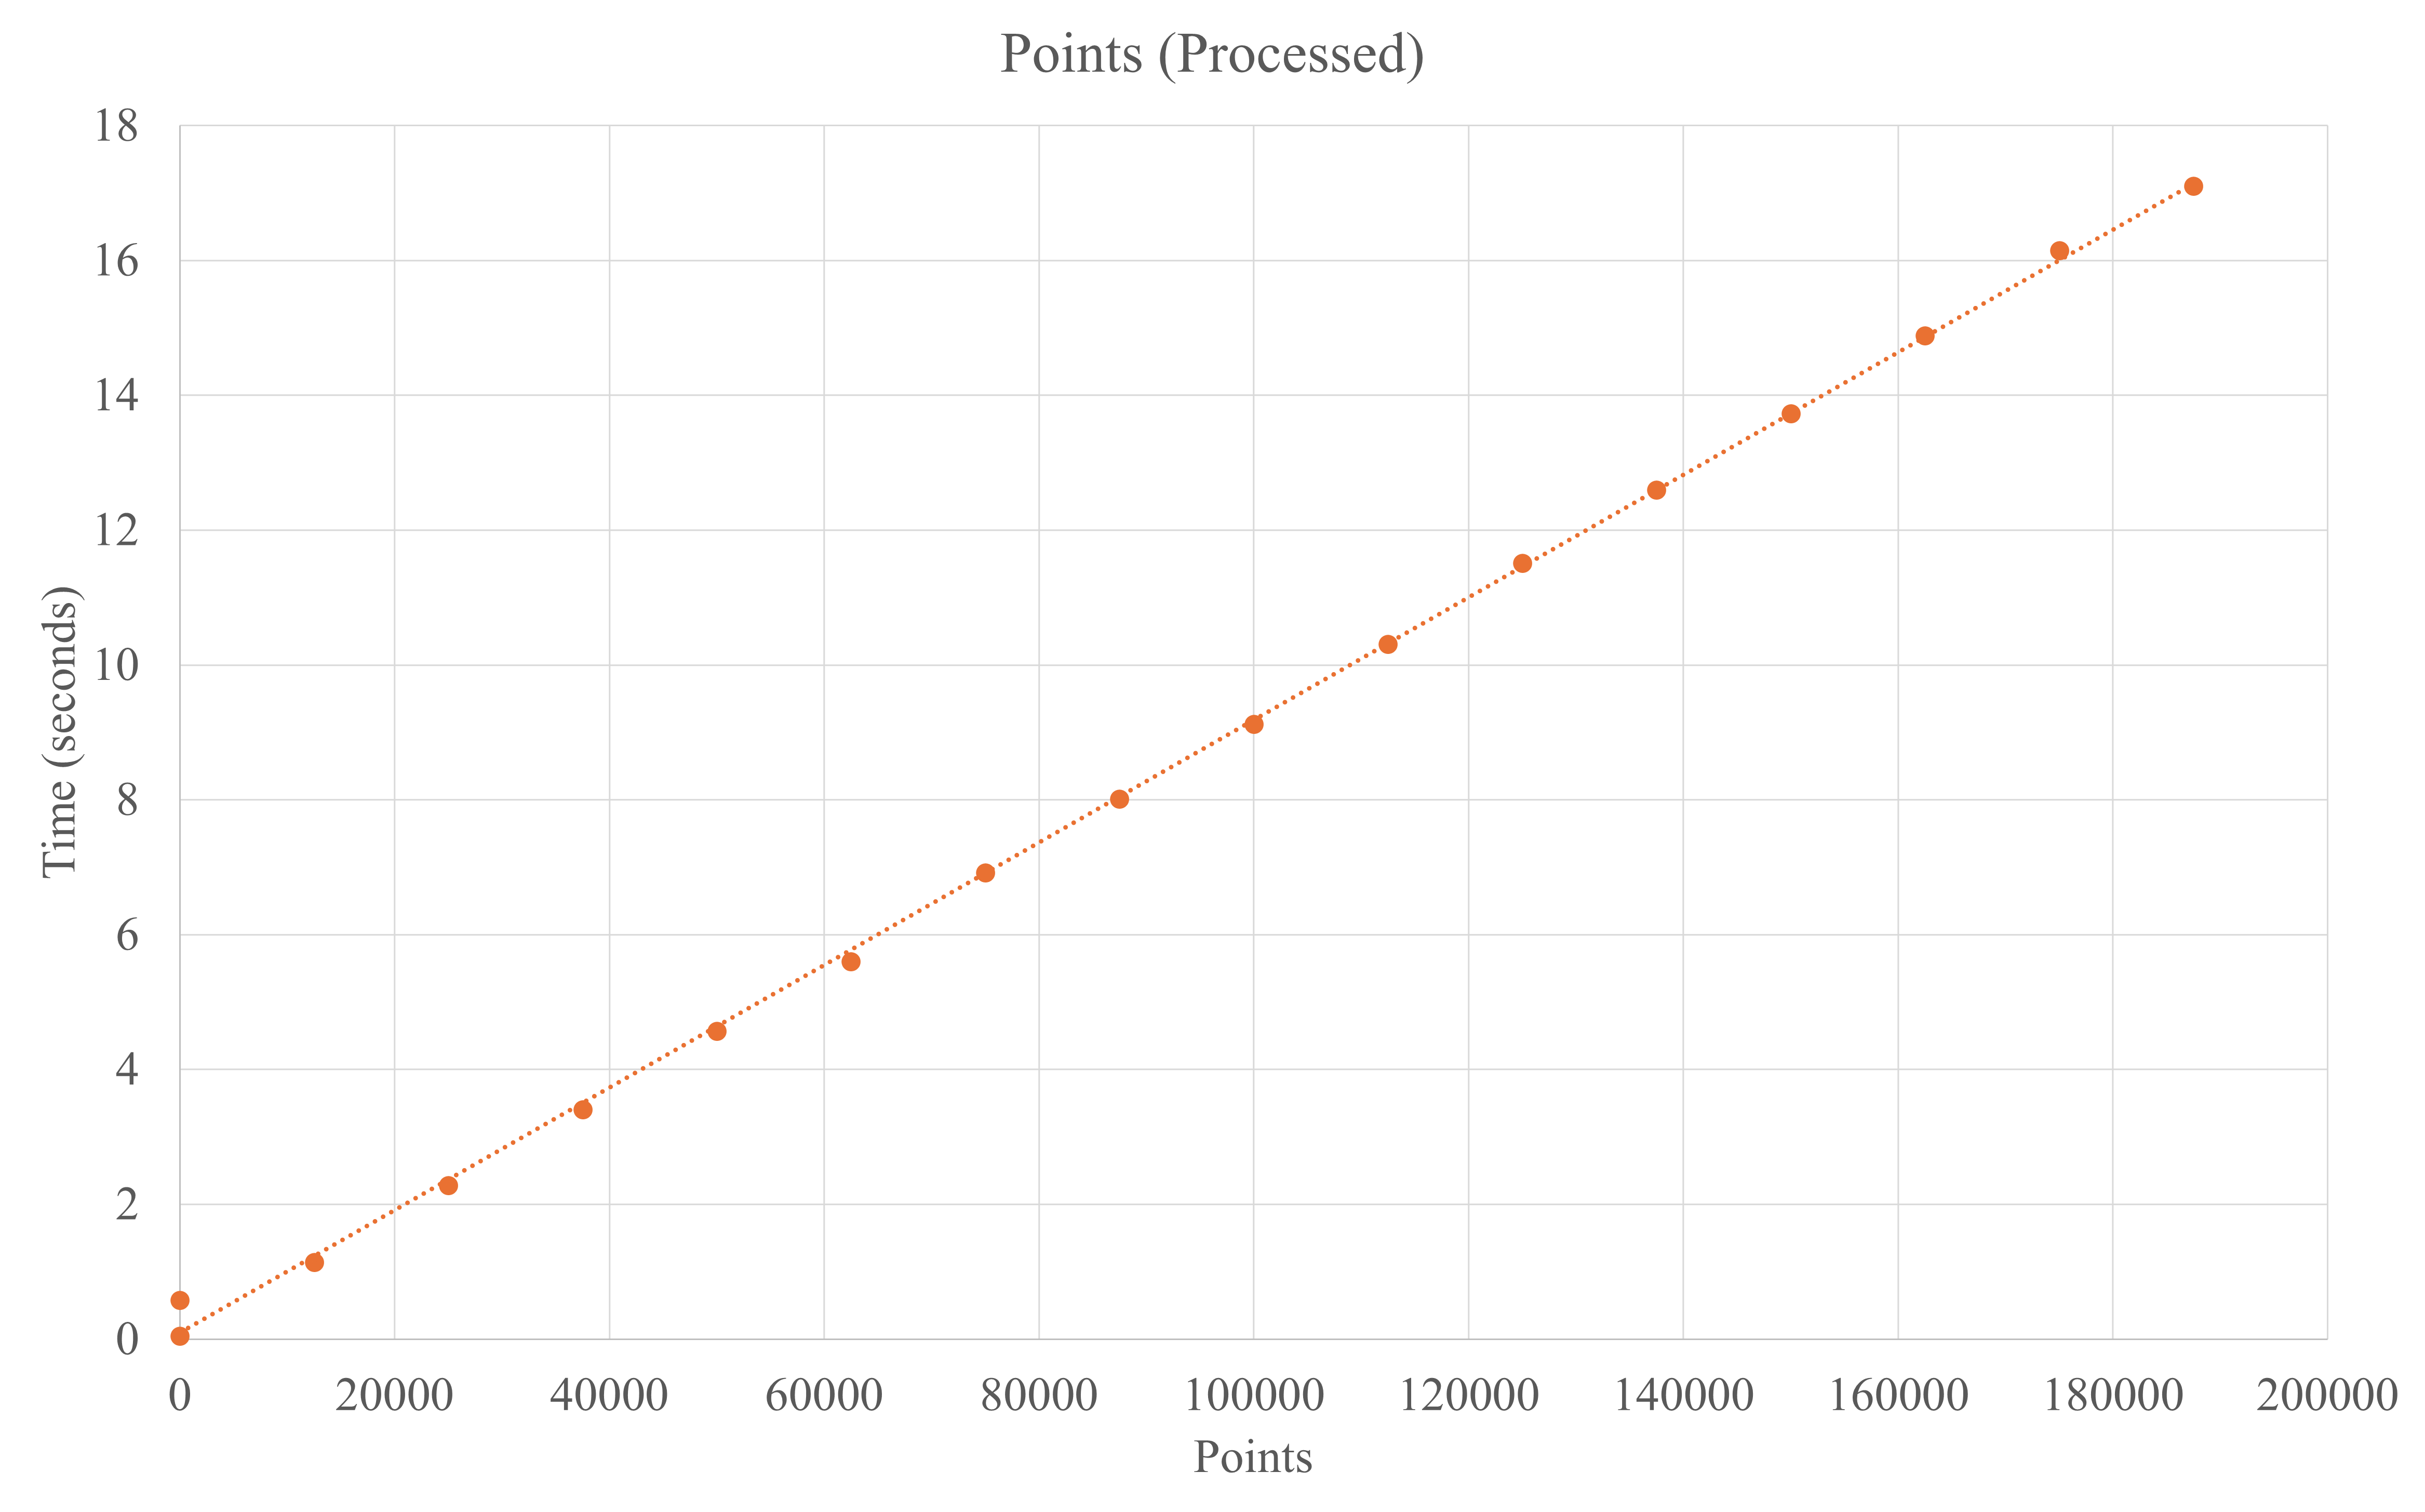
\includegraphics[width=0.45\linewidth]{PointsEdited.png}}
    \end{tabular}
    \caption{Runtime for increasing Points}
    \label{fig:PointsResults}
\end{figure}

\begin{figure}[h!]
    \centering
    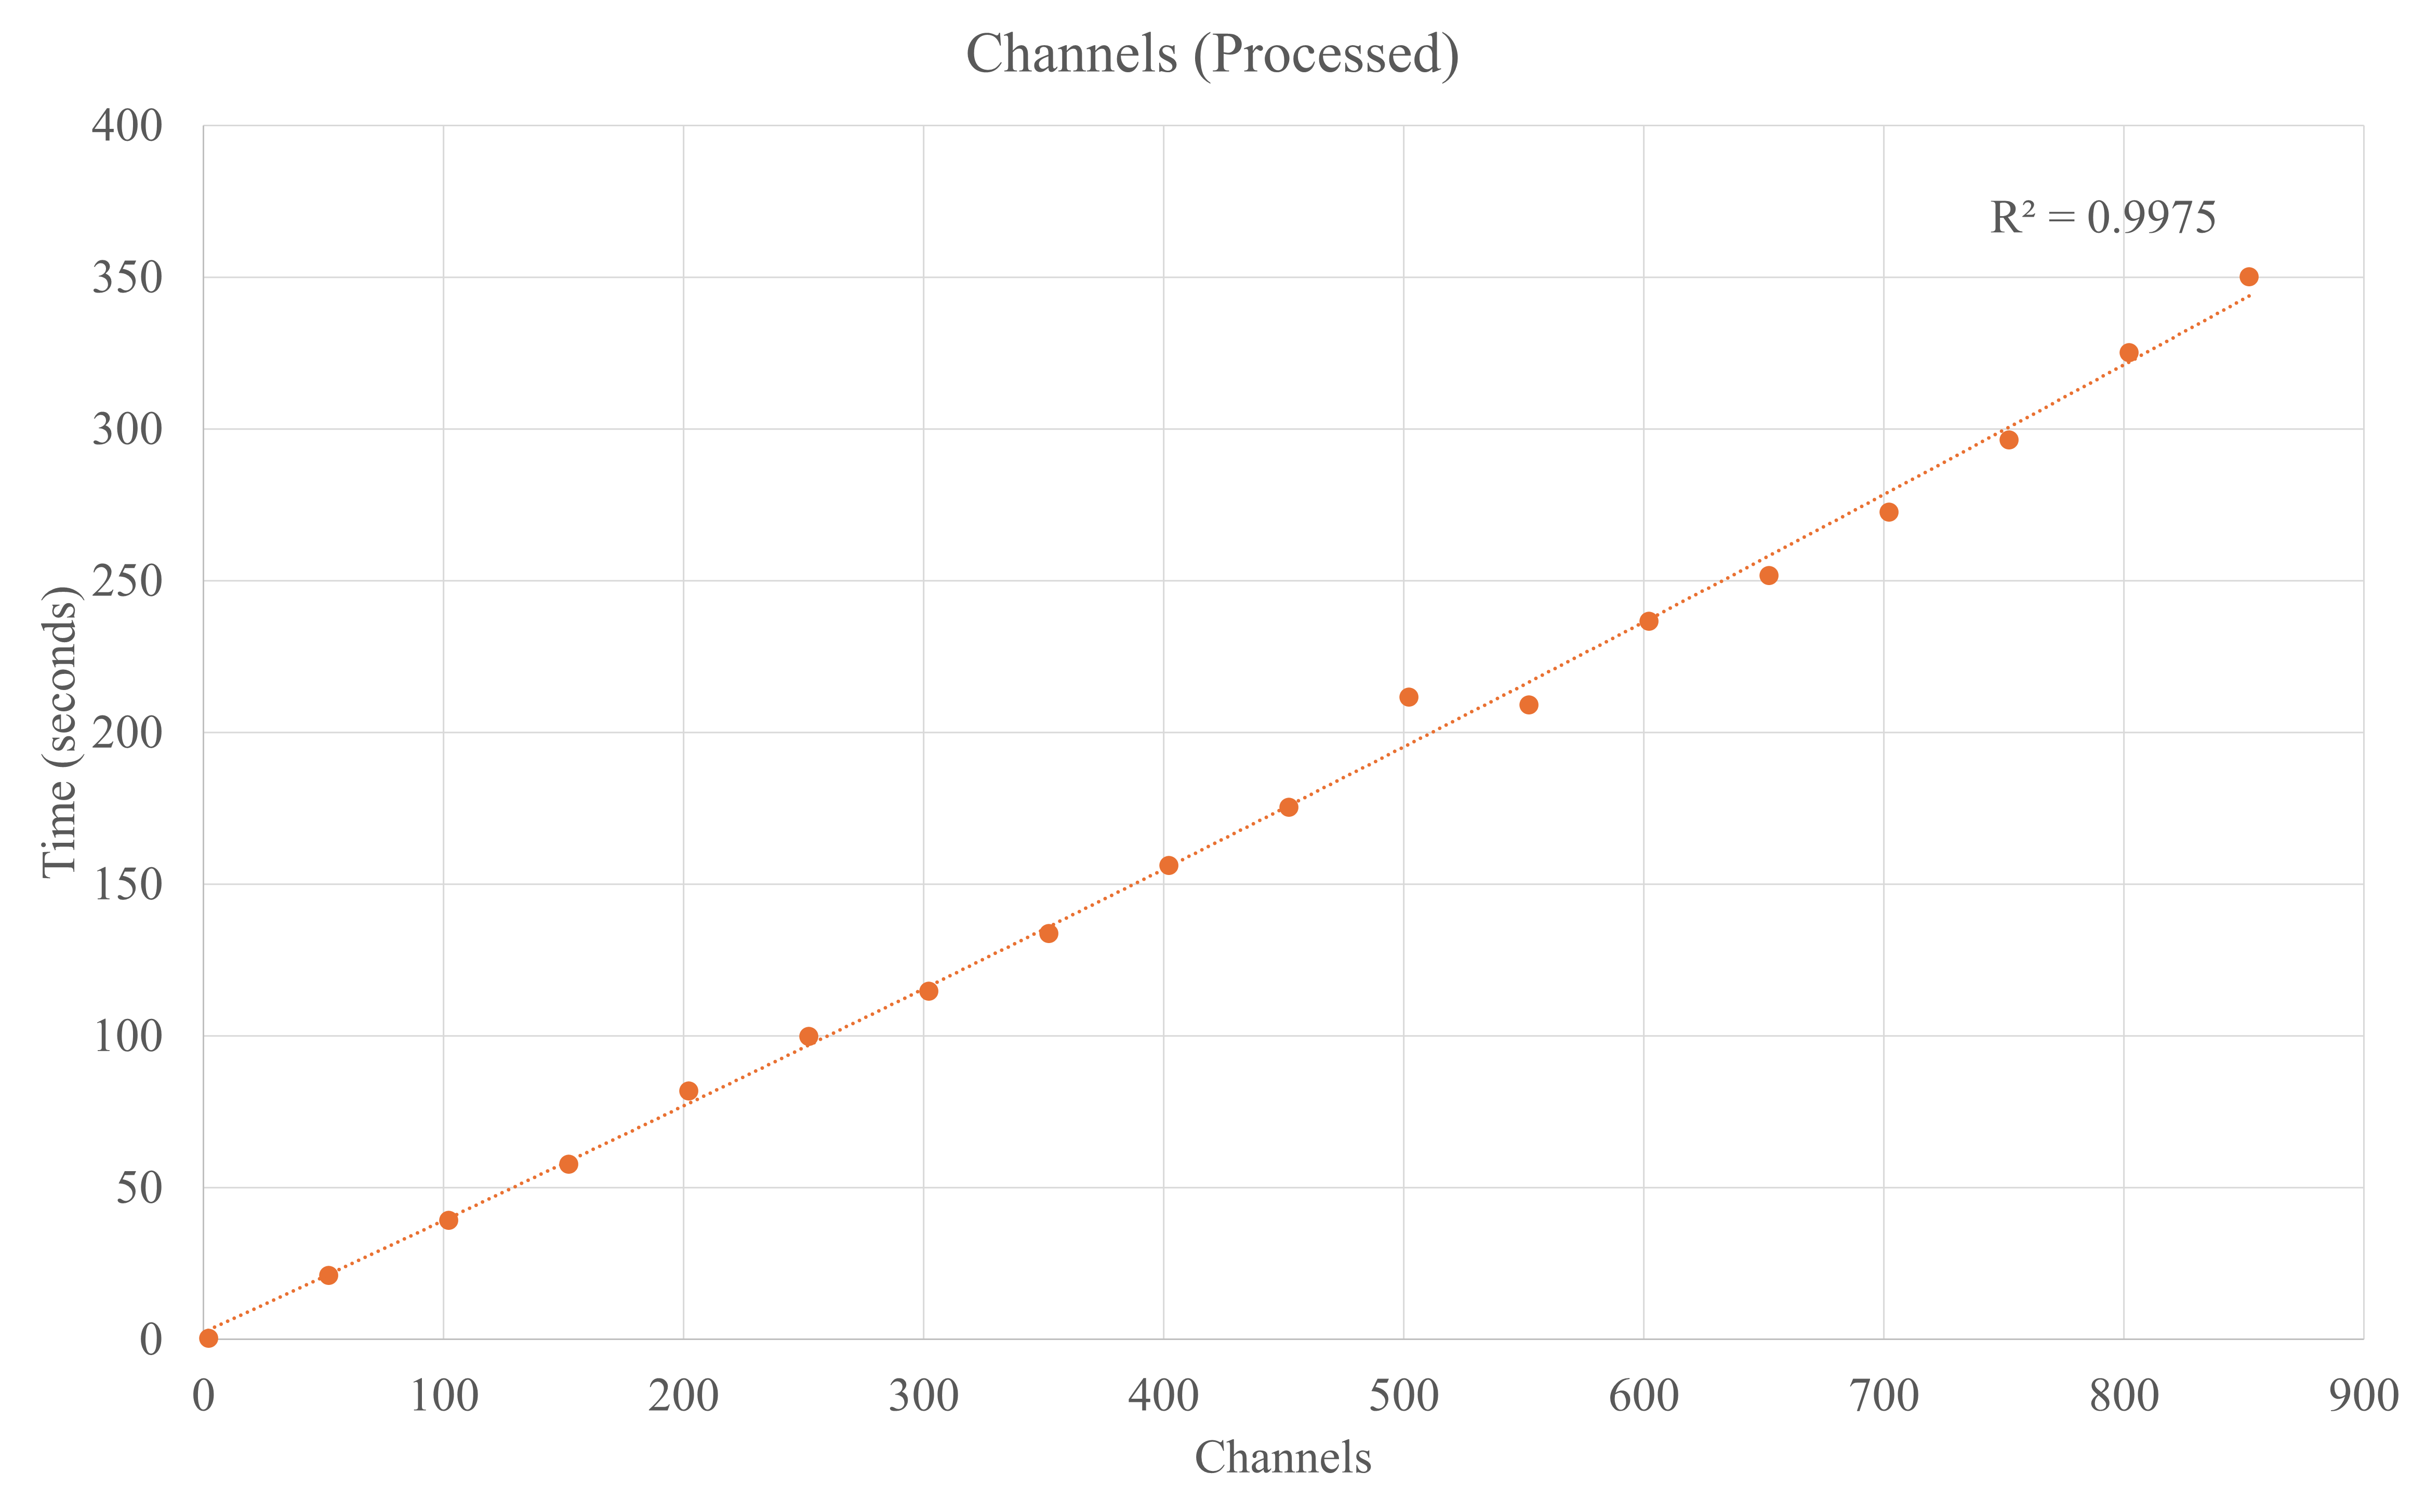
\includegraphics[width=0.75\linewidth]{ChannelsUnedited.png}
    \caption{Runtime for increasing Channels}
    \label{fig:ChannelsResults}
\end{figure}
\vspace{1mm}
\begin{figure}[h!]
    \begin{tabular}{cc}
        \subfloat[Unedited Frequencies]{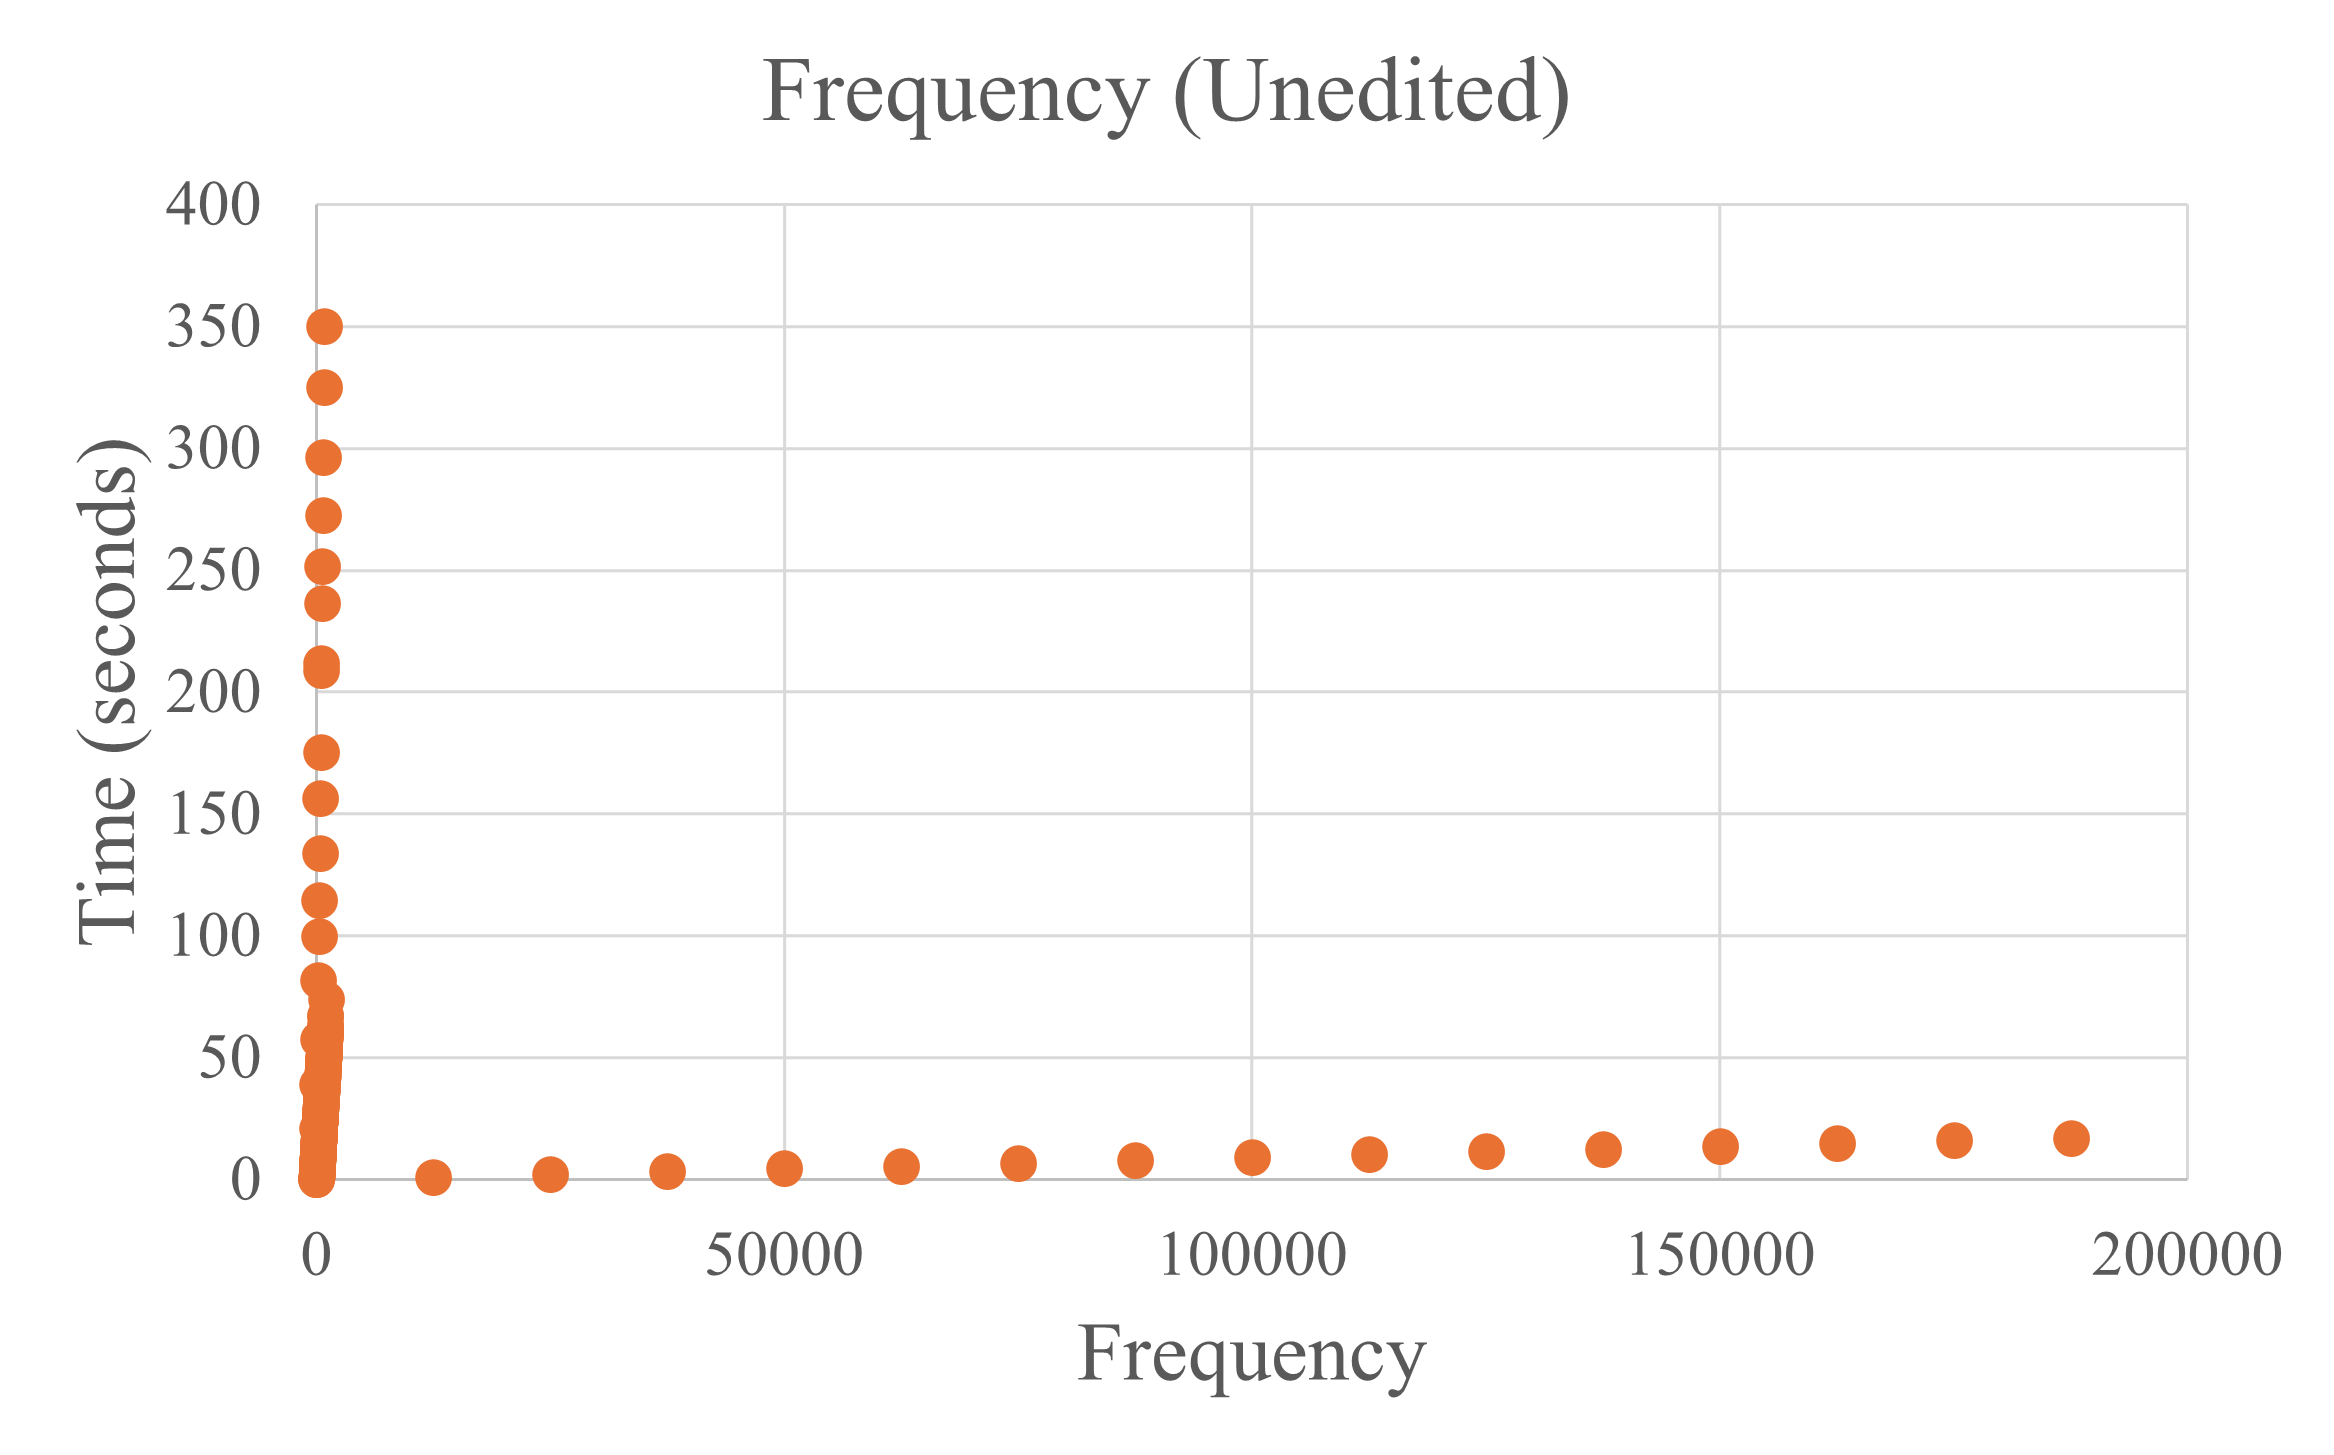
\includegraphics[width=0.45\linewidth]{FrequencyUnedited.png}}&
        \subfloat[Edited Frequencies]{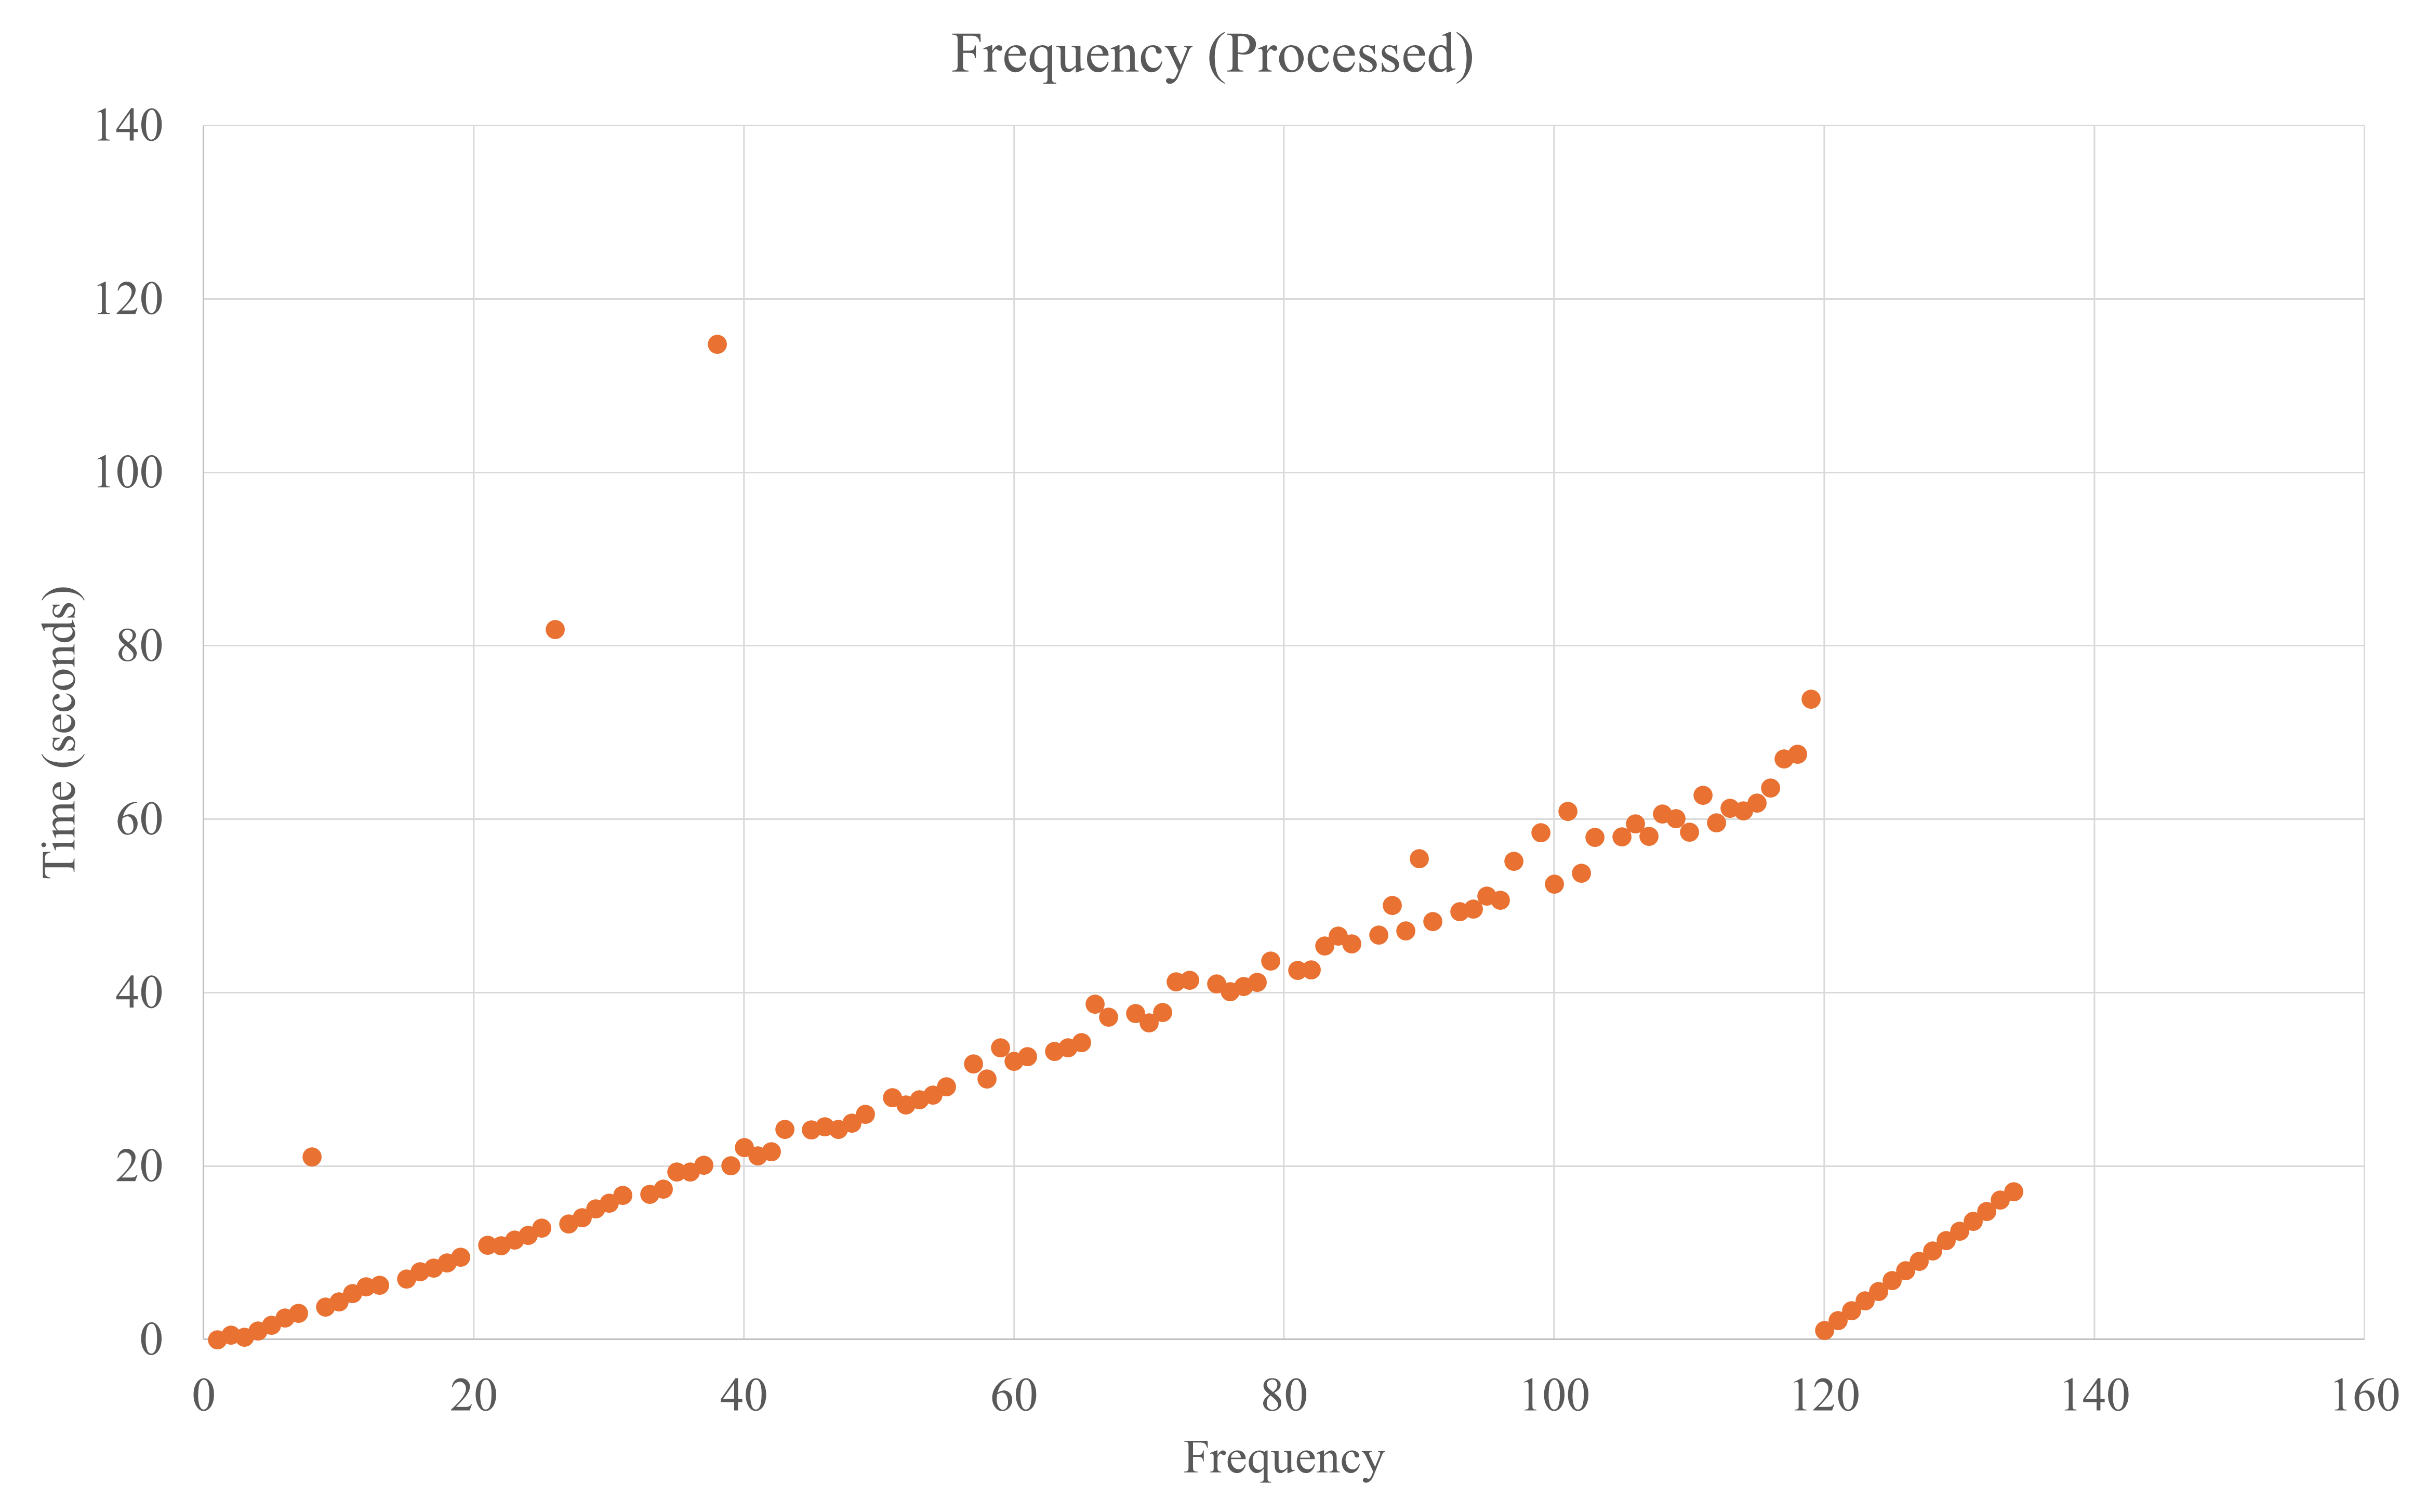
\includegraphics[width=0.45\linewidth]{FrequencyEdited.png}}
    \end{tabular}
    \caption{Runtime for increasing Frequency divisions}
    \label{fig:FrequenciesResults}
\end{figure}

Shown above in Figures \ref{fig:PointsResults}, \ref{fig:ChannelsResults}, \ref{fig:FrequenciesResults} are the results
from BenchmarkTools. The reason for the two types of graphs was to remove outliers that skewed the data and prohibited
any analysis. Running the benchmark used all the free RAM available on my laptop as well as significant amounts of swap
space on my drive due to large amounts of overhead introduced by the BenchmarkTools benchmark. I believe that the
latency caused by IO to the swap file was the cause for the outliers and so I removed them in the edited graphs since
these points are not indicative of the actual performance of the library. After these points were removed, a curve was
fitted to each graph to provide an indication of the time complexity. From this analysis, I concluded that the runtime
of the library scales linearly ($\mathcal{O}(n)$) with the number of points, and quadratically ($\mathcal{O}(n^2)$) with
the number of channels. This aligns with expectations based on the code analysis of the DAS implementation. The main
beamformer loop consists of a single for loop iterating over the points as such, the algorithm is expected to behave
linearly with an increase in points. With channels, every additional antenna corresponds to a quadratic increase in
channels since every antenna can send to and receive from any other antenna in a fully multistatic system. This is
evidenced by the slight quadratic increase in Figure \ref{fig:ChannelsResults}. The algorithm is expected to have
$\mathcal{O}(n)$ growth since the frequency is only used once in the algorithm process to delay each signal, which is
evidenced by the linear growth in \ref{fig:FrequenciesResults}. Effectively, MERIT works very well with a large number
of points and with relatively few channels. This in turn affected the layout of the matrices in the library. Since data
to do with points would be accessed most frequently, the decision was made to place these along the columns of the
matrices. Since Julia is a column major language, this would provide the quickest access to this data. Data that relate
to the channels were placed along the second dimension since this would be accessed less frequently than data related to
the points. Finally, data relating to the frequency were placed along the third dimension, since this data is accessed
very infrequently, it was decided that the latency required to load this data from memory would be acceptable provided
it allowed us easy access to data relating to points and channels. The above graphs demonstrate the performance of the
MERIT.jl library. From limited testing on my laptop with an Intel i7-1185G7 CPU and 16GB of RAM, the Julia library
executed in the same amount of time as its MATLAB counterpart. However, further testing to accurately quantify the
runtime of both libraries is needed.